\section{Experiments}
\label{experiments}


Our experiments share a common animation platform (our Experiment Setup) and a common Data Collection protocol.  Our experiments differ in presenting subjects with a range of Experimental Conditions.  All of the experiments described in this section together with the methods that we have chosen to analyze the data were based on a private but approved pre-registration on \textit{aspredicted.org}. The document is publicly available at \url{https://aspredicted.org/cg753.pdf}.


% \footnote{Pre-registration on https://aspredicted.org/ on 08/25/2019. The document is publicly available at \url{https://aspredicted.org/cg753.pdf}.} 


\subsection{Experiment Setup}
Each animation shows a simulated robot producing two pointing gestures to specify a pick-and-place task.  Following the animation, viewers are asked whether a specific image represents a possible result of the specified task.\\

\noindent\textbf{Robotic Platforms} The experiments were performed on two different robotic geometries, based on a \textit{Rethink Baxter}, and a \textit{Kuka IIWA14}.  The \textit{Baxter} is a dual-arm manipulator with two arms mounted on either side of a static torso. The experiments only move the right arm of the \textit{Baxter}. The \textit{Kuka}  consists of a single arm that is vertically mounted, i.e., points upward at the base. In the experiments the robots are shown with a singly fingered tool-tip, where the pointing ray is modeled as the direction of this tool-tip.

\noindent\textit{Note} The real Baxter robot possesses a heads-up display that can be likened to a `head'. This has been removed in the simulations that were used in this study (as shown for example in Figure~\ref{fig:natural}).\\

\noindent\textbf{Workspace Setup} Objects are placed in front of the manipulators. In certain trials a table is placed in front of the robot as well, and the objects rest in stable configurations on top of the table. A pick-and-place task is provided specified in terms of the positions of one of the objects. \\

\noindent\textbf{Objects}  The objects used in the study include small household items like mugs, saucers and boxes (cuboids), that are all placed in front of the robots.\\

\noindent\textbf{Motion Generation}  The end-effector of the manipulator is instructed to move to pre-specified waypoints, designed for the possibility of effective communication, that typically lie between the base of the manipulator and the object itself. Such waypoints fully specify both the position and orientation of the end-effector to satisfy \textit{pointing actions}. The motions are performed by solving Inverse Kinematics for the end-effector geometry and moving the manipulator along these waypoints using a robotic motion planning library 
\cite{pracsys2014}.
The motions were replayed on the model of the robot, and rendered in \textit{Blender}.\\


\begin{figure}[t]
    \centering
    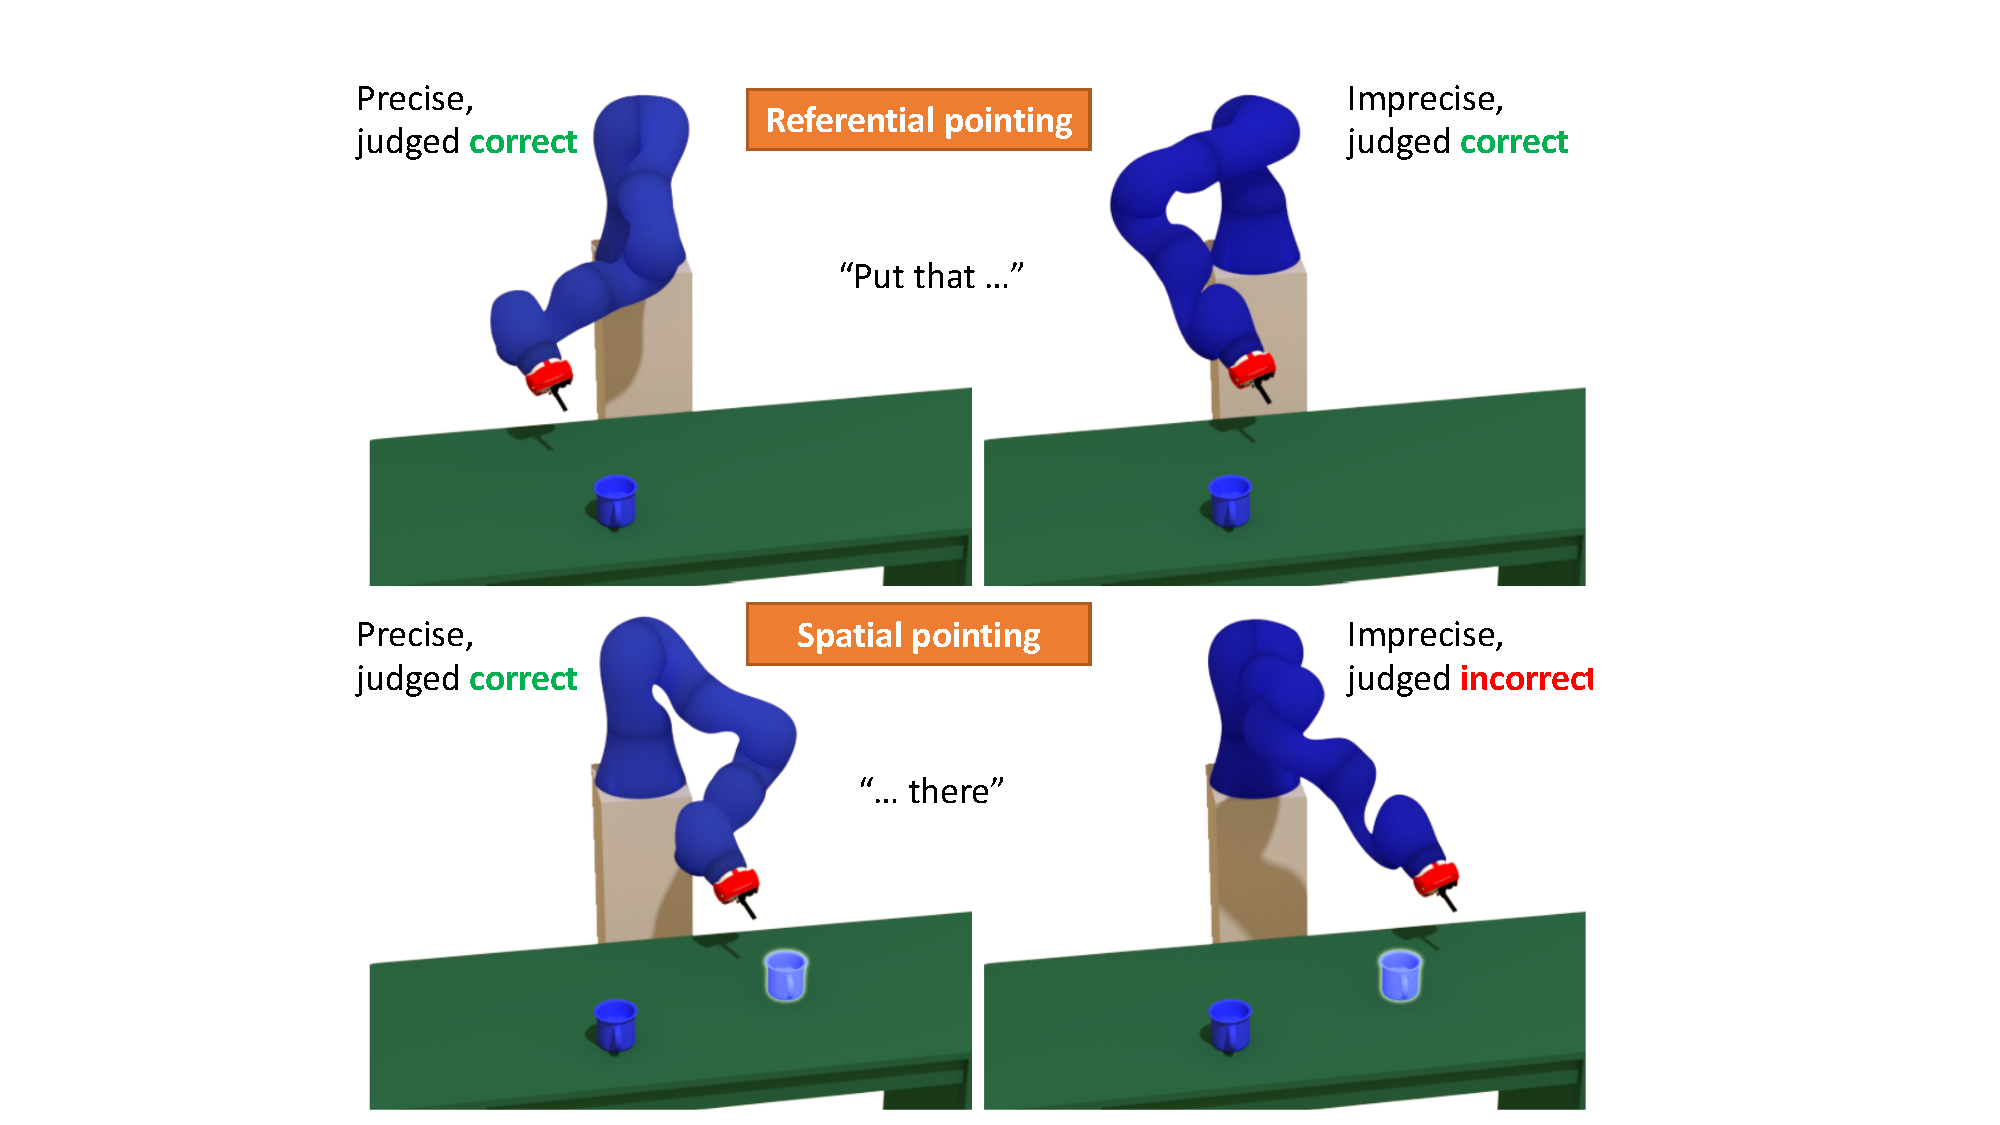
\includegraphics[width=0.48\textwidth]{spatial-referential.pdf}
    \caption{The image shows the differences between referential (\textit{top}) and locating pointing (\textit{bottom}), demonstrated on a robotic manipulator, \textit{Kuka IIWA14}. An overlay of the object is shown at the placement location where locating pointing needs to be directed.  Human subjects are more flexible in the interpretation of  referential pointing than with that of locating pointing.}
    \label{fig:spatial}
\end{figure}

\noindent\textbf{Pointing Action Generation} Potential pointing targets are placed using a cone $C(r, \theta)$, where $r$ represents the pointing ray and $\theta$ represents the vertex angle of the cone. As illustrated in Fig~\ref{fig:pointing}, the cone allows us to assess the possible divergence between the pointing ray and the actual location of potential target objects on the rest surface $S$. 

Given a pointing ray $r$, we assess the resolution of the pointing gesture by sampling $N$ object poses $p_i, i=1:N$ in $P=C(r, \theta) \cap S$---the intersection of the pointing cone with the rest surface.  While $p_i$ is the 6d pose for the object with translation $t \in R^3$ and orientation $R \in SO(3)$ only 2  degrees-of-freedom $(x, y)$ corresponding to $t$ are varied in the experiments. By fixing the $z$ coordinate for translation and restricting the z-axis of rotation to be perpendicular to $S$, it is ensured that the object rests in a physically stable configuration on the table.

The $N$ object poses are sampled by fitting an ellipse within $P$ and dividing the ellipse into 4 quadrants $q_1\ldots q_4$ (See Figure~\ref{fig:pointing} (C)). Within each quadrant $q_i$ the $N/4$ $(x,y)$ positions are sampled uniformly at random. For certain experiments additional samples are generated with an objective to increase coverage of samples within the ellipse by utilizing a dispersion measure.\\

\noindent\textbf{Speech} Some experiments also included verbal cues with phrases like `\textit{Put that there}' along with the pointing actions. It was very important for the pointing actions and these verbal cues to be in synchronization. To fulfill this we generate the voice using Amazon Polly with text written in SSML format and make sure that peak of the gesture (the moment a gesture comes to a stop) is in alignment with the peak of each audio phrase in the accompanying speech. During the generation of the video itself we took note of the peak moments of the gestures and then manipulated the duration between peaks of the audio using SSML to match them with gesture peaks after analyzing the audio with the open-source tool PRAAT (www.praat.org).



\begin{figure}[t]
    \centering
    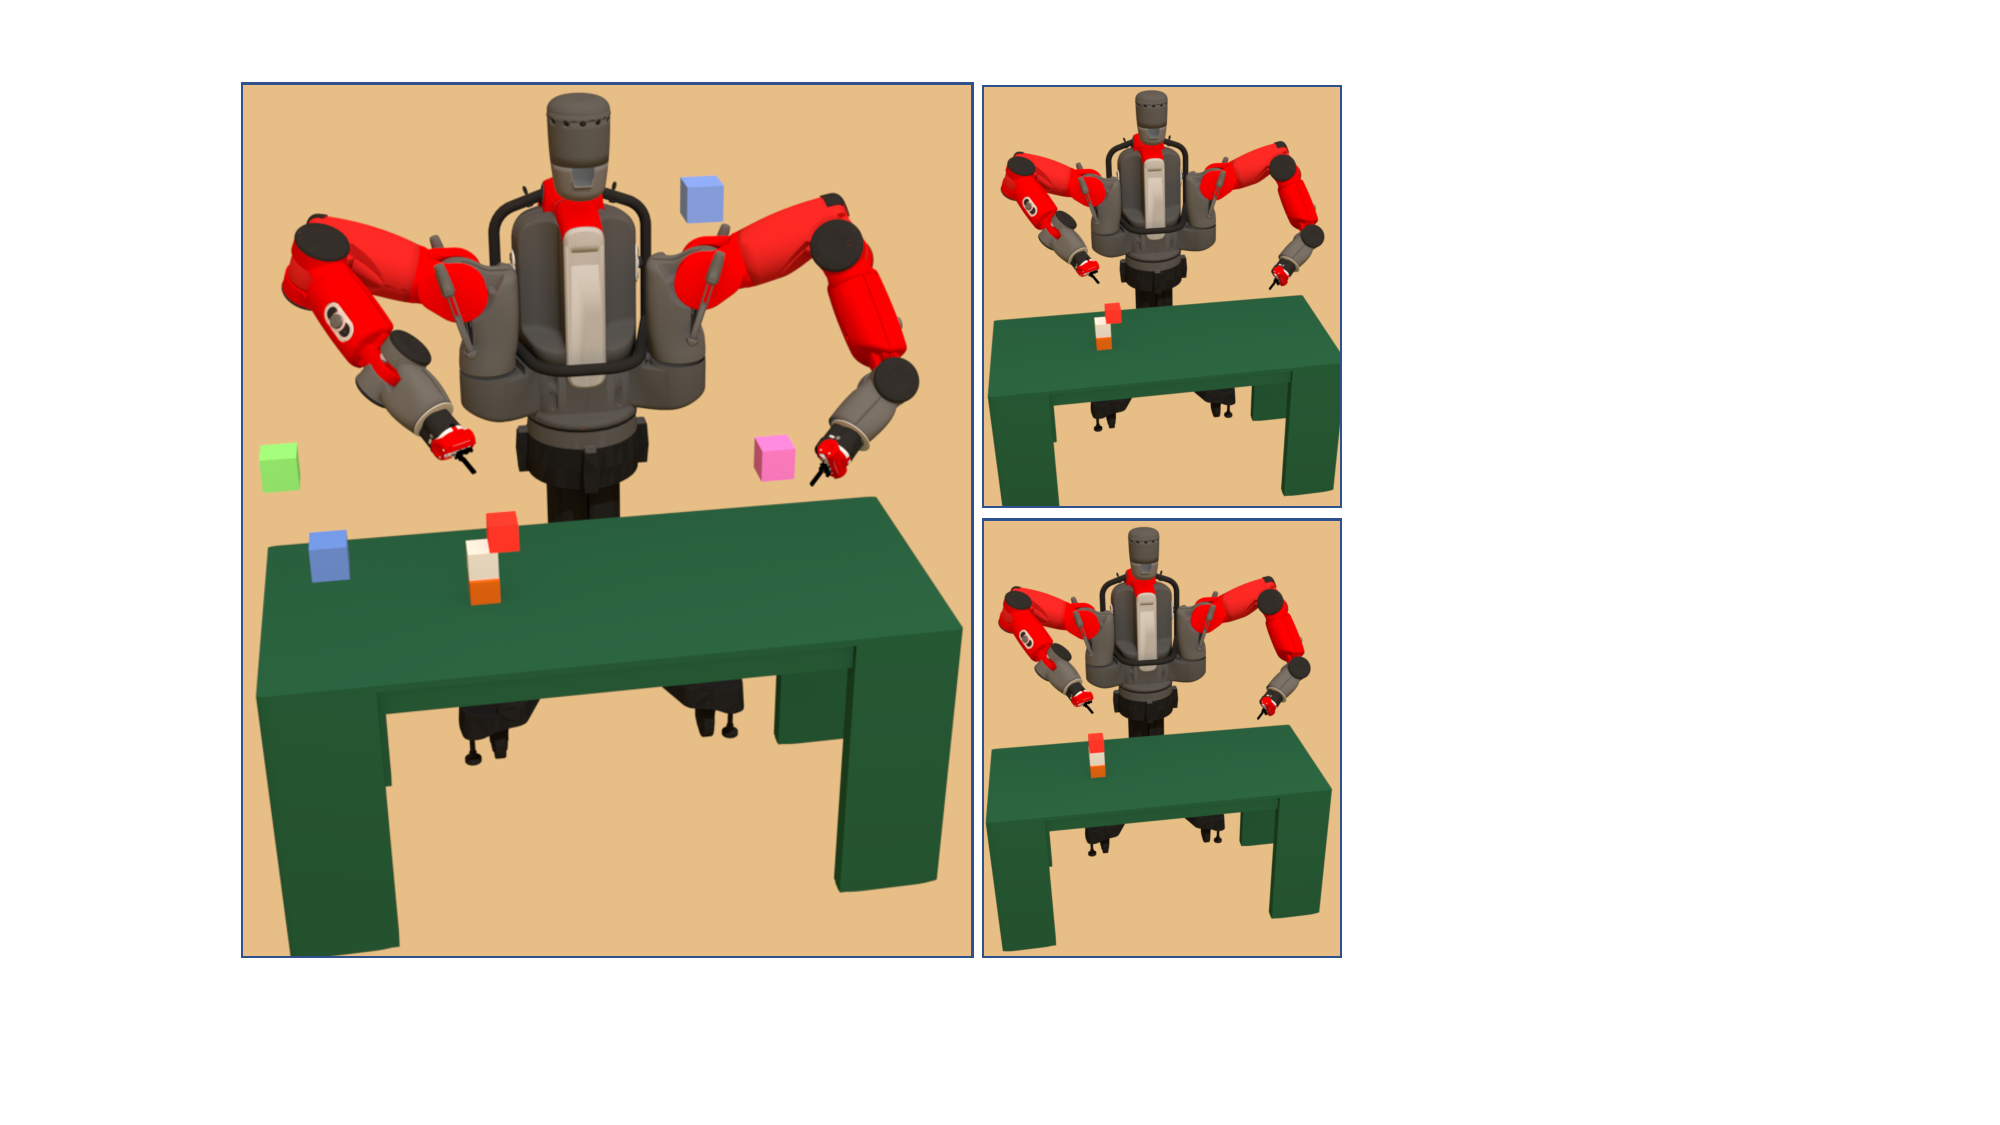
\includegraphics[width=0.45\textwidth]{natural.pdf}
    \caption{(Left) In an unnatural scene, a gesture pointing to an unstable position (edge of the stack) is deemed correct. (Right) In natural scenes, although the robot points to the edge of the stack, a physically realistic object position gets more user vote than the unstable position.}
    \label{fig:natural}
\end{figure}

\subsection{Data Collection}

Data collection was performed in \textit{Amazon Mechanical Turk}. All subjects agreed to a consent form and were compensated at an estimated rate of \textit{USD 20} an hour. The subject-pool was restricted to non-colorblind US citizens. Subjects are presented a rendered video of the simulation where the robot performs one referential pointing action, and one locating pointing action which amounts to it pointing to an object, and then to a final location. During these executions synchronized speech is included in some of the trials to provide verbal cues.

Then on the same page, subjects see the image that shows the result of the pointing action. They are asked whether the result is (a) correct, (b) incorrect, or (c) ambiguous.  

To test our hypothesis, we studied the interpretation of the two pointing behaviors in different contexts. Assuming our conjecture and a significance level of 0.05, a sample of 28 people in each condition is enough to detect our effect with a 95\% power.  Participants are asked to report judgments on the interpretation of the pointing action in each class.  Each participant undertakes two trials from each class.  The range of different cases are described below.  Overall, the data collection in this study involved over 7,290 responses to robot pointing actions. \footnote{ The data, code, and videos are available at  \url{https://github.com/malihealikhani/That_and_There}.}

\subsection{Experimental Conditions}

We used our experiment setup to generate videos and images from the simulation for a range of different conditions.

\paragraph{Referential vs Locating}
In this condition, to reduce the chances of possible ambiguities, we place only one mug is on the table. The \textit{Baxter} robot points its right arm to the mug and then points to its final position, accompanied by a synchronized verbal cue, \textit{``Put that there.''}

We keep the motion identical across all the trials in this method. 
We introduce a variability in the initial position of the mug by sampling $8$ random positions within conic sections subtending $45^{\circ} , 67.5^{\circ}, $ and $90^{\circ}$ on the surface of the table. New videos are generated for each such position of the mug.
This way we can measure how flexible subjects are to the variation of the initial location of the referent object. 

To test the effect for the locating pointing action, we test similarly sampled positions around the final pointed location, and display these realizations of the mug as the result images to subjects, while the initial position of the mug is kept perfectly situated. 

A red cube that is in the gesture space of the robot, and is about twice as big as the mug is placed on the other side of the table as a visual guide for the subjects to see how objects can be placed on the table. We remove the tablet that is attached to Baxter's head for our experiments.\\ 

\noindent\textit{Effect of speech} In order to test the effect of speech on the disparity between the kinds of pointing actions, a set of experiments were designed under the \textit{Referential vs Locating} method with and without any speech. All subsequent methods will include verbal cues during their action execution. These cues are audible in the video.

\paragraph{Reverse Task} One set of experiments are run for the pick-and-place task with the initial and final positions of the object flipped during the reverse task. As opposed to the first set of experiments, the robot now begins by pointing to an object in the middle of the table, and then to an area areas towards the table's edge, i.e., the pick and place positions of the object are `reversed'. 

The trials are meant to measure the sensitivity of the subjects in pick trials to the direction of the pointing gestures and to the absolute locations that the subjects thought the robot was pointing at.


This condition is designed to be identical to the basic Referential vs Locating study, except for the direction of the action. The motions are still executed on the \textit{Baxter's} right arm. 

\paragraph{Different Robotic Arm}
In order to ensure that the results obtained in this study are not dependent on the choice of the robotic platform or its visual appearance, a second robot---a singly armed industrial \textit{Kuka} manipulator---is also evaluated in a Referential vs Locating study (shown in Figure~\ref{fig:spatial}).


\begin{figure}[t]
    \centering
    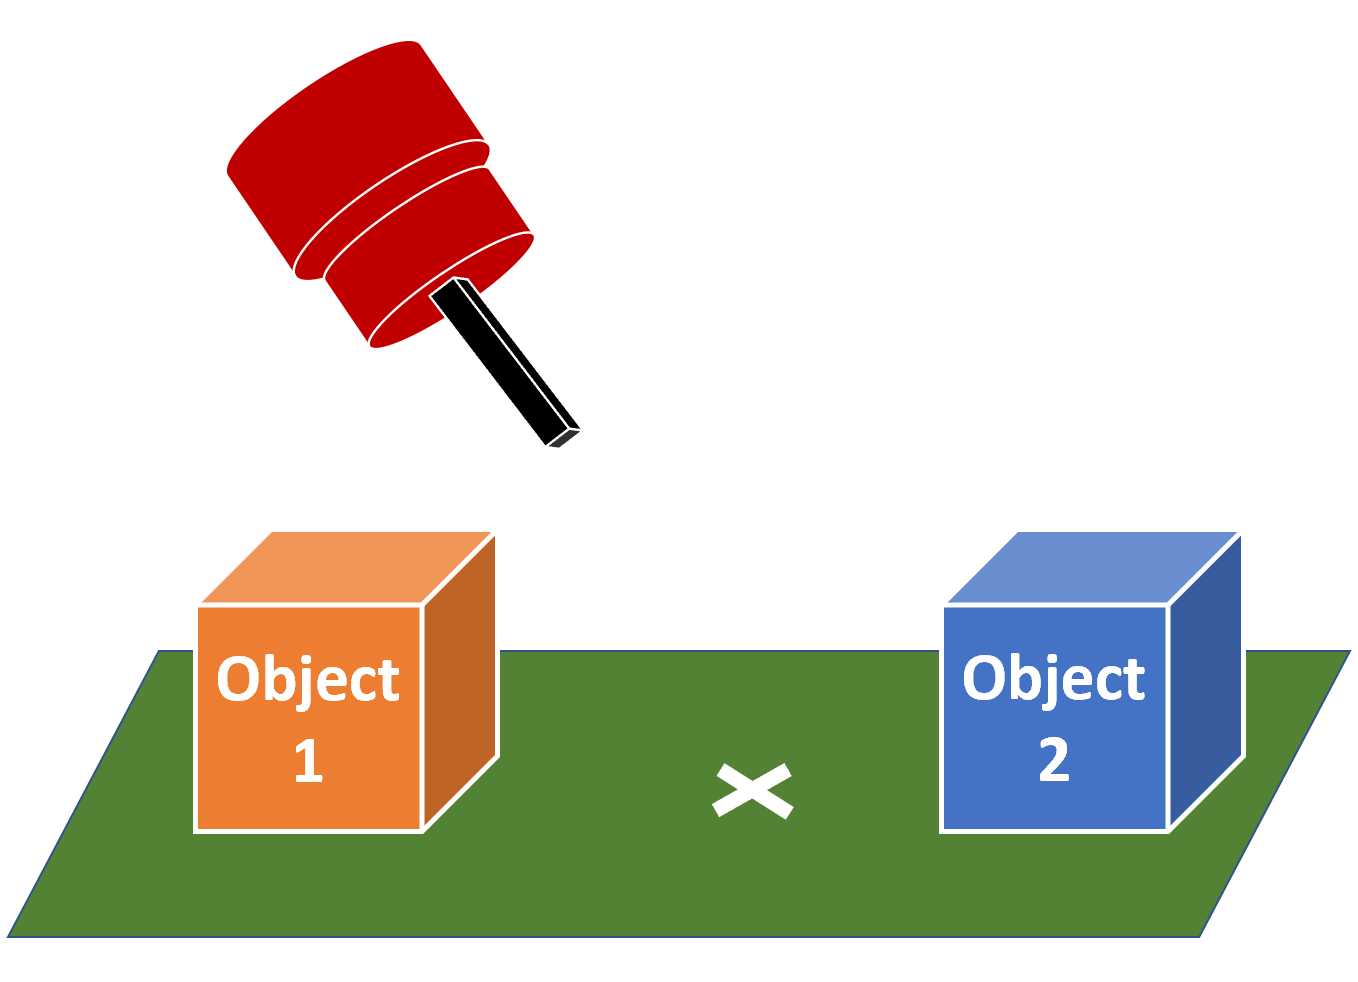
\includegraphics[width=0.40\textwidth]{figures/clutter_trial.png}
    \caption{A cluttered trial consists of collecting the response from a human subject when the position of the referential pointing action lies between two objects.}
    \label{fig:cluttered_trial}
\end{figure}


\paragraph{Cluttered Scene}
To study how the presence of other objects would change the behavior of referential pointing, we examine the interpretation of the pointing actions when there is more than one \textit{mug} on the table. Given the instructions to the subjects, both objects are candidate targets. This experiment allows the investigation of the effect of a distractor object in the scene on referential pointing.  

We start with a setup where there are two mugs placed on the table (similar to the setup in Figure~\ref{fig:cluttered_trial}). One is a target mug placed at position $\xobject$ and a distractor mug at position $\xdistractor$. With the robot performing an initial pointing action to a position $\xinit$ on the table. Both the objects are sampled around $\xinit$ along the diametric line of the conic section arising from increasing cone angles of $45^\circ, 67.5^\circ, $ and $90^\circ$, where the separation of $\xobject$, and $\xdistractor$ is equal to the length of the diameter of the conic section, $D$. The objects are then positioned on the diametric line with a random offset between $[-\frac{D}{2}, \frac{D}{2}]$ around $\xinit$ and along the line. This means that the objects are at various distances apart, and depending upon the offset, one of the objects is nearer to the pointing action. The setup induces that the nearer mug serves as the \textit{object}, and the farther one serves as the \textit{distractor}. The motions are performed on the \textit{Baxter's} right arm. The camera perspective in simulation is set to be facing into the pointing direction. The subjects in this trial are shown images of the instant of the referential pointing action.


\paragraph{Natural vs Unnatural scene}
In this condition we study how the contextual and physical understanding of the world impacts the interpretation of pointing gestures. We generate a scenario for locating pointing in which the right arm of the \textit{Baxter} points to a final placement position for the cuboidal object on top of a stack of cuboidal objects but towards the edge which makes it physically unstable. The final configurations of the object (Figure~\ref{fig:topedgetable}) shown to the users were a) object lying on top of the stack b) object in the unstable configuration towards the edge of the stack and c) object at the bottom of the stack towards one side. New videos are generated for each scenario along with verbal cues.

The pointing action, as well as the objects of interest, stay the identical between the natural, and unnatural trials. The difference lies in other objects in the scene that could defy gravity and float in the unnatural trials. The subjects were given a text-based instruction at the beginning of an unnatural trial saying they were seeing a scene where ``gravity does not exist.'' 


\begin{figure}[h!]
    \centering
    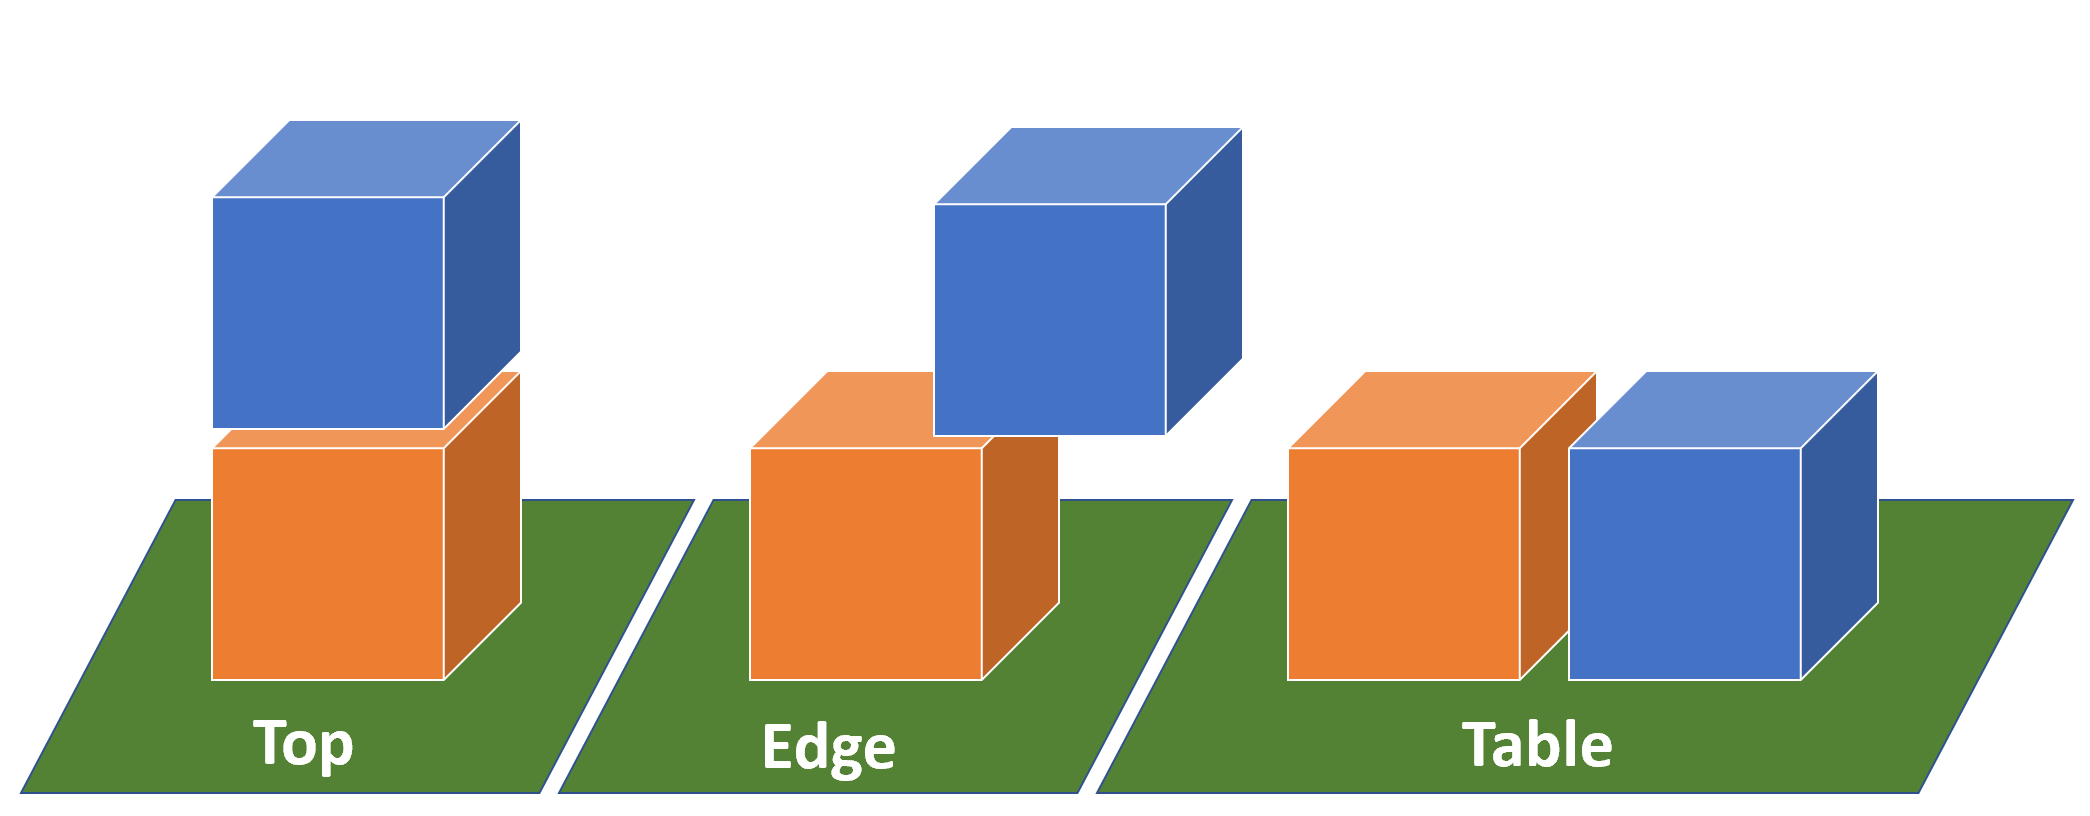
\includegraphics[width=0.47\textwidth, trim={0 0 0 0.7in},clip ] {figures/topedgetable.png}
    % \vspace{-0.1in}
    \caption{
    The diagram shows the three different configurations of the placement of a blue cuboid object evaluated in the \textit{Natural vs Unnatural} trials. 
    }
    \label{fig:topedgetable}
\end{figure}


\paragraph{Different verbs}  
To test if the effect is specific to the verb \textit{put}, we designed a control condition where everything remained the same as the Referential vs Locating trials except the verb \textit{put} which we replaced with \textit{place, move} and \textit{push}. Here again we collect 30 data points for each sampled $x^*$.

